%Corps du document :
%\setlength{\parindent}{1cm}    

\section{Cadre du projet}

Le but du projet ``Système d'Information Urbanisé et SOA'' est de mettre en application la démarche et
les méthodes de conception de systèmes d'information vues en cours dans le cadre d'une architecture répartie.

\subsection{Thème du projet}

Il s'agira de fournir une solution logicielle pour ``la gestion des contacts commerciaux'' d'une banque,
en apportant une aide à ses agents commerciaux pour :

\begin{itemize}
\item Identifier et définir les contacts qu'ils doivent avoir avec leurs clients,
\item Permettre au chef d'agence de répartir ces contacts entre ses collaborateurs,
\item Prendre les rendez-vous et tenir leurs agendas,
\item Préparer ces rendez-vous et les projets de proposition en fonction des clients,
\item Construire les entretiens lors des rendez-vous et déclarer les résultats obtenus,
\item Suivre la réalisation des contacts programmés.
\end{itemize}

\subsection{Phases du projet}

Ce projet se déroulera en 3 phases :

\begin{itemize}
\item La conception d'ensemble de l'architecture applicative,
\item La conception détaillée des applications,
\item La répartition des composants sur l'architecture n-tiers.
\end{itemize}

\subsection{Outils de suivi}

\begin{itemize}
\item Nous utiliserons l'outil de gestion de projet \textbf{RedMine} pour la conduite de projet, la répartition et l'organisation des tâches, et l'établissement d'un planning prévisionnel.
\item Notre RedMine sera interfacé avec l'outil de gestion de révision \textbf{Git} pour le suivi de l'évolution des documents et son environnement de travail collaboratif distribué.
\end{itemize}

\subsection{Objectifs en termes de produits finis}

\begin{itemize}
\item Document d'Initialisation
\item Compte-Rendu du projet :

\begin{itemize}
\item Conception d'ensemble
\item Conception détaillée
\item Architecture de l'application
\end{itemize}

\item Présentation orale
\item Bilan du projet
\end{itemize}

\section{Organisation des tâches}

\subsection{Répartition des tâches}

\begin{itemize}
\item Conception d'ensemble du système

\begin{itemize}
\item Analyse des modèles conceptuels proposés (assigné à \textbf{Xavier Sauvagnat})
\item Etablissement des diagrammes d'activités (assigné à \textbf{Matthieu Coquet})
\item Etablissement des diagrammes de séquences systèmes (assigné à \textbf{Alexandre Lefoulon})
\item Identifier et définir les blocs applicatifs

\begin{itemize}
\item Etablissement du modèle de données découpés en blocs (assigné à \textbf{Alexandre Lefoulon})
\end{itemize}

\item Identifier les cycles de vie des objets métiers

\begin{itemize}
\item Etablissement du diagramme d'état d'objet métier, objet Contact UNIQUEMENT (assigné à \textbf{Jan Keromnes})
\end{itemize}

\item Détermination des flux de l'architecture

\begin{itemize}
\item Etablissement d'un diagramme de séquence (assigné à \textbf{Quentin Calvez})
\item Etablissement d'un diagramme de collaboration(assigné à \textbf{Thaddee Tyl})
\end{itemize}

\item Choix de l'environnement technique (assigné à \textbf{Matthieu Coquet})

\end{itemize}
\item Conception détaillée

\begin{itemize}
\item Interface utilisateur

\begin{itemize}
\item Diagrammes EdF (assigné à \textbf{Jan Keromnes})
\item Description des fenêtres (assigné à \textbf{Quentin Calvez})
\item Services IHM (assigné à \textbf{Jan Keromnes})
\end{itemize}

\item Couche noyau

\begin{itemize}
\item Spécification des SM (assigné à \textbf{Xavier Sauvagnat})
\item Spécification des SOM (assigné à \textbf{Alexandre Lefoulon})
\end{itemize}

\end{itemize}

\item Architecture technique et répartition du SI

\begin{itemize}
\item Choix architecture Centralisée/Réparties (assigné à \textbf{Quentin Calvez})
\item Choix de la répartition des composants applicatifs (assigné à \textbf{Thaddee Tyl})
\item Détermination des principaux flux au sein de l'application, CRUD (assigné à \textbf{Jan Keromnes})
\end{itemize}

\end{itemize}

\subsection{Evaluation des charges}

\begin{itemize}
\item Conception d'ensemble du système

\begin{itemize}
\item Analyse des modèles conceptuels proposés (temps estimé \textbf{2h00})
\item Etablissement des diagrammes d'activités (temps estimé \textbf{3h00})
\item Etablissement des diagrammes de séquences systèmes (temps estimé \textbf{2h00})

\item Identifier et définir les blocs applicatifs

\begin{itemize}
\item Etablissement du modèle de données découpés en blocs (temps estimé \textbf{2h00})
\end{itemize}

\item Identifier les cycles de vie des objets métiers

\begin{itemize}
\item Etablissement du diagramme d'état d'objet métier, objet Contact UNIQUEMENT (temps estimé \textbf{1h00})
\end{itemize}

\item Détermination des flux de l'architecture

\begin{itemize}
\item Etablissement d'un diagramme de séquence (temps estimé \textbf{2h00})
\item Etablissement d'un diagramme de collaboration(temps estimé \textbf{2h00})
\end{itemize}

\item Choix de l'environnement technique (temps estimé \textbf{2h00})

\end{itemize}

\item Conception détaillée

\begin{itemize}
\item Interface utilisateur

\begin{itemize}
\item Diagrammes EdF (temps estimé \textbf{4h00})
\item Description des fenêtres (temps estimé \textbf{4h00})
\item Services IHM (temps estimé \textbf{1h00})
\end{itemize}

\item Couche noyau

\begin{itemize}
\item Spécification des SM (temps estimé \textbf{3h00})
\item Spécification des SOM (temps estimé \textbf{3h00})
\end{itemize}

\end{itemize}

\item Architecture technique et répartition du SI

\begin{itemize}
\item Choix architecture Centralisée/Réparties (temps estimé \textbf{3h00})
\item Choix de la répartition des composants applicatifs (temps estimé \textbf{3h00})
\item Détermination des principaux flux au sein de l'application, CRUD (temps estimé \textbf{3h00})
\end{itemize}

\end{itemize}


\section{Diagramme de Gantt}

\begin {center}
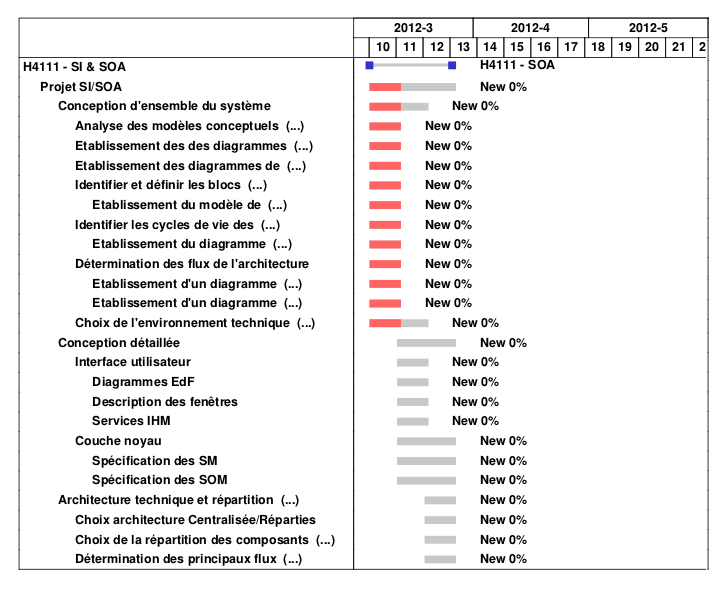
\includegraphics[width=\textwidth]{gantt.png}
\end {center}
